\documentclass[10pt]{standalone}
\usepackage{amsmath}
\usepackage{amssymb}
\usepackage{pgf,tikz}
\usepackage{mathrsfs}
\usetikzlibrary{arrows}
\pagestyle{empty}

\begin{document}

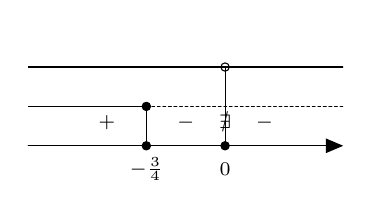
\begin{tikzpicture}[line cap=round,line join=round,>=triangle 45,x=1.0cm,y=1.0cm]

\draw[->] (0.5,0.) -- (4.5,0.);
\
\clip(0.5,-0.5) rectangle (4.5,1.5);
\draw (0.5,0.5)-- (2.,0.5);
\draw [dash pattern=on 1pt off 1pt] (2.,0.5)-- (4.5,0.5);
\draw (2.,0.5)-- (2.,0.);
\draw (3.,1.)-- (3.,0.);
\draw (0.5,1.)-- (4.5,1.);
\begin{scriptsize}
\draw [fill=black] (2.,0.) circle (1.5pt);
\draw[color=black] (2.0,-0.3) node {$-\frac{3}{4}$};
\draw[color=black] (1.5,0.3) node {$+$};
\draw[color=black] (2.5,0.3) node {$-$};
\draw[color=black] (3.5,0.3) node {$-$};
\draw [fill=black] (3.,0.) circle (1.5pt);
\draw[color=black] (3.0,-0.3) node {$0$};
\draw[color=black] (3.0,0.3) node {$\nexists$};
\draw  (3.,1.) circle (1.5pt);
\draw [fill=black] (2.,0.5) circle (1.5pt);
\end{scriptsize}
\end{tikzpicture}
\end{document}